\documentclass[root.tex]{subfiles}

\begin{document}

{\pagestyle{empty}}
\section{HiL-Architecture}
\label{chap:HiL-Architecture}
\gls{VTM} includes a lot of processing-heavy sub-models (tire models, vehicle parameter sets) which lead to processing power not sufficing to allow for \gls{VTM}'s execution in the dSpace environment on the \gls{MABII}. To perform \gls{HIL}-testing it was thus necessary to split the computational load and accomplish real-time data exchange between the hardware controlling-system on the \gls{MABII} and the rest of the simulation which will be run parallely in Simulink in real-time on a standard PC. Though there are dedicated real-time platforms available to achieve real-time execution it was decided to rely on a standard PC to minimize costs and have a lean work-process without extra steps of code conversion to different platforms. Figure \ref{fig:HIL_overview} illustrates the distribution of the \gls{HIL}-setup's different components according to the Volvo GTT functionality model over two computers, the \gls{MABII} and the actual hardware. The \gls{VMM} consists of the controller previously developed which is executed on the Simulation-PC and the steering interface executed on the \gls{MABII}. For track-testing it of course is necessary to also port the controller for execution on the \gls{MABII} to have one closed of system. This was not yet possible to achieve for the tests at hand, as some blocks used within the controller-algorithm's  Simulink were incompatible for real-time execution on the dSpace system.

\begin{figure*}[h]
	\centering
	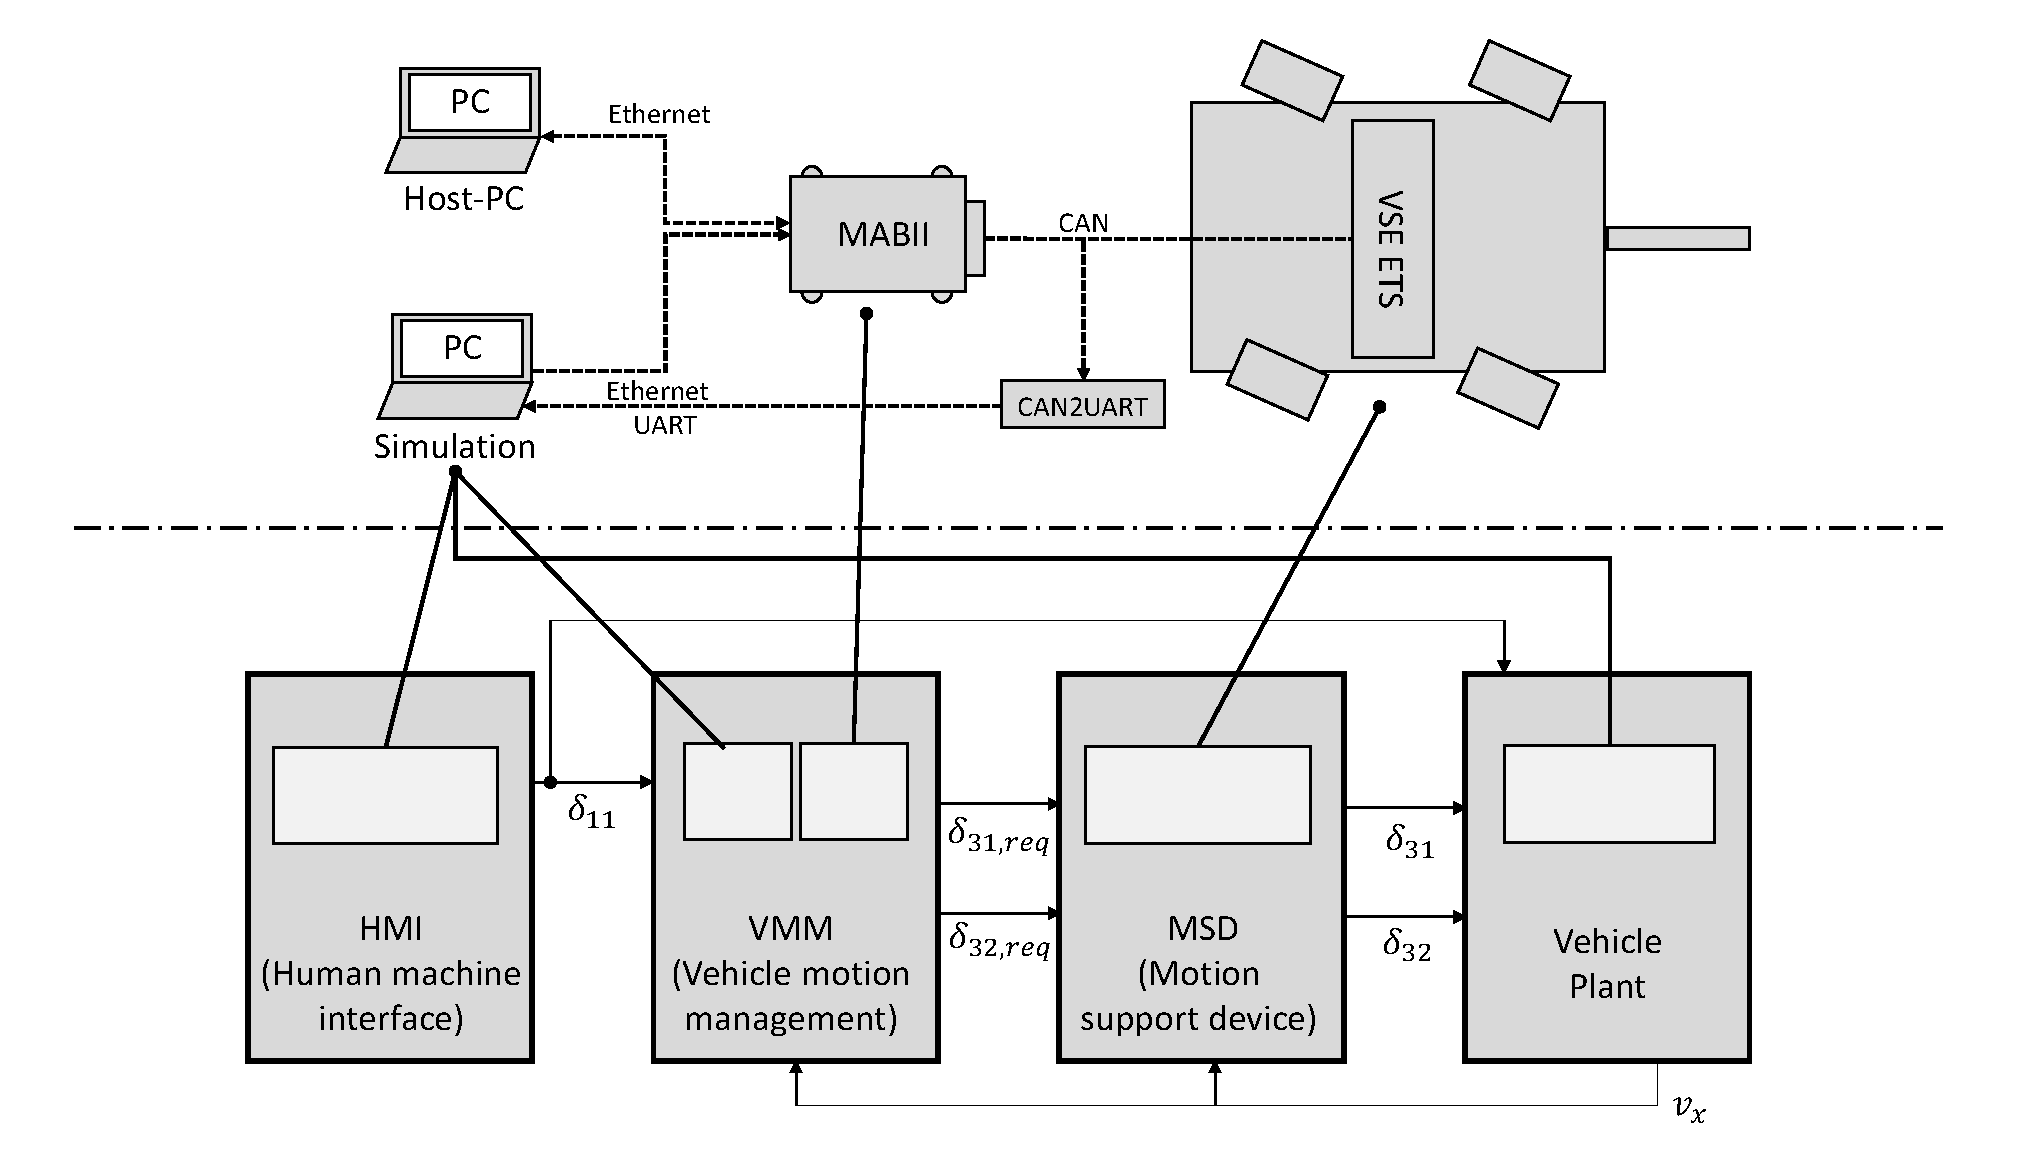
\includegraphics[width=0.8\linewidth]{HIL_overview}
	\caption[Overview of \acrlong{HIL}-simulation, distribution of sub-functions over different physical platforms (top) and correlation to Volvo functionality architecture (bottom)]{Overview of \gls{HIL}-simulation, distribution of sub-functions over different physical platforms (top) and correlation to Volvo functionality architecture (bottom)}
	
	\label{fig:HIL_overview}
\end{figure*}
\end{document}